\documentclass[11pt, letterpaper]{article}

% Fonts and Encoding
\usepackage[utf8]{inputenc}
\usepackage[T1]{fontenc}
\usepackage{lmodern} % High-quality Latin Modern vector font

% Math and Symbols
\usepackage{amsmath, amssymb, amsthm, amsfonts, mathrsfs, mathtools}

% Layout and Geometry
\usepackage{geometry}
\geometry{letterpaper, margin=1in}
\setlength{\parindent}{0pt}
\setlength{\parskip}{0.6em}

% Formatting and Graphics
\usepackage{graphicx, xcolor, enumitem, booktabs, array, tabularx}

% TikZ for Illustrations
\usepackage{tikz}
\usetikzlibrary{arrows.meta, positioning, shapes.geometric, calc, backgrounds, matrix}

% Clickable Links and TOC
\usepackage{hyperref}
\hypersetup{
    colorlinks=true,
    linkcolor=blue,
    filecolor=magenta,      
    urlcolor=cyan,
    pdftitle={Advanced Mathematics Topic},
}

% Theorem Environments
\newtheorem{theorem}{Theorem}[section]
\newtheorem{lemma}[theorem]{Lemma}
\newtheorem{proposition}[theorem]{Proposition}
\newtheorem{corollary}[theorem]{Corollary}
\theoremstyle{definition}
\newtheorem{definition}{Definition}[section]
\newtheorem{axiom}{Axiom}[section]
\newtheorem{example}{Example}[section]
\theoremstyle{remark}
\newtheorem{remark}{Remark}[section]

% Custom Commands (Enforced standard notation)
\newcommand{\R}{\mathbb{R}}
\newcommand{\N}{\mathbb{N}}
\newcommand{\Z}{\mathbb{Z}}
\newcommand{\Q}{\mathbb{Q}}
\newcommand{\E}{\mathbb{E}}
\newcommand{\Prob}{\mathbb{P}}
\newcommand{\F}{\mathcal{F}}

\begin{document}

\title{Advanced Abstract Mathematics: Functions, Mappings, and Rigorous Probability Models\\
\large Comprehensive Practice Problem Set}
\author{Tashfeen Omran}
\date{\today}
\maketitle

\tableofcontents
\newpage

\section{Concept Checklist \& Question Mapping}

The following table maps the core theoretical concepts extracted from the source text to the 30 rigorous problems generated in this document.

\renewcommand{\arraystretch}{1.5}
\begin{tabularx}{\textwidth}{>{\raggedright\arraybackslash}p{1.5cm} >{\raggedright\arraybackslash}X >{\raggedright\arraybackslash}p{3.5cm}}
\toprule
\textbf{ID} & \textbf{Concept / Logical Structure} & \textbf{Associated Problems} \\
\midrule
C1 & Relation vs. Function (Existence \& Uniqueness) & 1, 2, 3, 4 \\
C2 & Domain and Range Computations (Algebraic Inversion) & 5, 6, 7, 8 \\
C3 & Image and Preimage Properties (Set-Theoretic Proofs) & 9, 10, 11, 12 \\
C4 & Cardinality of Function Spaces ($|B^A|$) & 13, 14, 15 \\
C5 & Higher-Order Functions and Functionals ($C^{B^A}$) & 16, 17, 18 \\
C6 & Injectivity, Surjectivity, and Bijectivity & 19, 20, 21 \\
C7 & Composition of Functions & 22, 23, 24 \\
C8 & Abstract Real-World Modeling (Quant Finance \& ML) & 25, 26, 27, 28 \\
C9 & Flaw Identification / Diagnostic Logic & 29, 30 \\
\bottomrule
\end{tabularx}

\newpage

\section{Problem Sets}

\textbf{Part 1: Function Verification (Existence and Uniqueness)}
\begin{enumerate}[label=\textbf{\arabic*.}]
    \item Let $A = \Z$ and $B = \Z$. Define a relation $R$ from $A$ to $B$ by $xRy$ if and only if $y^2 = x^2$. Determine, with rigorous justification, whether $R$ is a function from $A$ to $B$.
    \item Let $A = \Q$ and $B = \Z$. Define a relation $R$ by $R = \left\{ \left(\frac{p}{q}, p+q\right) : p, q \in \Z, q \neq 0 \right\}$. Is $R$ a function? Prove your assertion.
    \item Let $S = \{n \in \N : n \ge 2\}$. Define a relation $R$ from $S$ to $S$ where $xRy$ if $y$ is the smallest prime factor of $x$. Prove that $R$ is a function.
    \item Let $A = \R$. Define $R \subseteq A \times A$ such that $(x, y) \in R \iff |x| + |y| = 1$. Is $R$ a function from $[-1, 1]$ to $\R$? Justify your answer.
\end{enumerate}

\textbf{Part 2: Domain and Range Computations}
\begin{enumerate}[label=\textbf{\arabic*.}, resume]
    \item Determine the domain and range of the function $f: D \to \R$ defined by $f(x) = \sqrt{\ln(x^2 - 3)}$. Express your answer in interval notation.
    \item Let $f(x) = \frac{e^x - e^{-x}}{e^x + e^{-x}}$. Find the maximal real domain $D \subseteq \R$ and rigorously compute the range of $f$ using algebraic inversion.
    \item Determine the range of $g(x) = \frac{4x}{x^2 + 1}$ over its maximal real domain.
    \item Let $h(x) = \ln(1 - \sin x)$. Find the domain $D \subseteq \R$ and the range of $h$.
\end{enumerate}

\textbf{Part 3: Image and Preimage Properties (Set-Theoretic Proofs)}
\begin{enumerate}[label=\textbf{\arabic*.}, resume]
    \item Let $f: X \to Y$ be a function, and let $A, B \subseteq X$. Prove that $f(A \cup B) = f(A) \cup f(B)$.
    \item Let $f: X \to Y$ be a function, and let $C, D \subseteq Y$. Prove that $f^{-1}(C \setminus D) = f^{-1}(C) \setminus f^{-1}(D)$.
    \item Prove that for any function $f: X \to Y$ and subsets $A, B \subseteq X$, $f(A \cap B) = f(A) \cap f(B)$ if and only if $f$ is injective.
    \item Let $f: X \to Y$ be a function and $A \subseteq X$. Prove that $A \subseteq f^{-1}(f(A))$. Provide a concrete counterexample to show that equality does not hold in general.
\end{enumerate}

\textbf{Part 4: Cardinality of Function Spaces}
\begin{enumerate}[label=\textbf{\arabic*.}, resume]
    \item Let $A = \{1, 2, 3, 4\}$ and $B = \{x, y, z\}$. How many functions exist in $B^A$? How many of these functions are surjective?
    \item Let $|A| = m$ and $|B| = n$ with $m \le n$. Derive the formula for the number of injective functions from $A$ to $B$.
    \item Let $A = \{0, 1\}$. Determine the cardinality of the set of all functions from $A^A$ to $A$. List two distinct elements of this higher-order function space.
\end{enumerate}

\textbf{Part 5: Higher-Order Functions and Functionals}
\begin{enumerate}[label=\textbf{\arabic*.}, resume]
    \item Let $\F(\R, \R)$ be the set of all functions from $\R$ to $\R$. Define the evaluation functional $\Phi_0: \F(\R, \R) \to \R$ by $\Phi_0(f) = f(0)$. Prove that $\Phi_0$ is surjective.
    \item Let $A, B, C$ be nonempty sets. Define a mapping $\Psi: C^B \times B^A \to C^A$ by $\Psi(g, f) = g \circ f$. Prove that if $|A|=|B|=|C|=1$, then $\Psi$ is a bijection.
    \item Let $S$ be a set. Define the indicator function $I_A: S \to \{0, 1\}$ for $A \subseteq S$. Prove that $I_{A \cap B}(x) = I_A(x) \cdot I_B(x)$ for all $x \in S$.
\end{enumerate}

\textbf{Part 6: Injectivity, Surjectivity, and Bijectivity}
\begin{enumerate}[label=\textbf{\arabic*.}, resume]
    \item Prove that the function $f: \R \setminus \{2\} \to \R \setminus \{3\}$ defined by $f(x) = \frac{3x + 1}{x - 2}$ is bijective.
    \item Prove that $f: \Z \times \Z \to \Z$ defined by $f(m, n) = 2m + 3n$ is surjective but not injective.
    \item Let $f: \R \to \R$ be defined by $f(x) = x^3 - 3x$. Prove rigorously that $f$ is neither injective nor surjective if restricted to the domain $[-1, 1]$.
\end{enumerate}

\textbf{Part 7: Composition of Functions}
\begin{enumerate}[label=\textbf{\arabic*.}, resume]
    \item Let $f: A \to B$ and $g: B \to C$ be functions. Prove that if $g \circ f$ is injective, then $f$ must be injective.
    \item Let $f: A \to B$ and $g: B \to C$. Prove that if $g \circ f$ is surjective, then $g$ must be surjective.
    \item Provide a concrete counterexample (using sets and mappings) to show that $g \circ f$ being injective does not imply $g$ is injective.
\end{enumerate}

\textbf{Part 8: Abstract Real-World Modeling (Quant Finance \& ML)}
\begin{enumerate}[label=\textbf{\arabic*.}, resume]
    \item \textbf{Quant Finance:} Let $(\Omega, \F, \Prob)$ be a probability space. A stock price $S_T: \Omega \to \R$ is a measurable function. A European Put Option payoff is $P(\omega) = \max(K - S_T(\omega), 0)$. Prove that the event ``the option expires in the money'' (i.e., $P(\omega) > 0$) is a measurable set in $\F$.
    \item \textbf{Quant Finance:} Let $V_0 = e^{-rT} \E^\Q[\max(S_T - K, 0)]$. Suppose $S_T(\omega) = K$ for all $\omega \in \Omega$. Rigorously evaluate $V_0$ and interpret the preimage $S_T^{-1}(\{K\})$.
    \item \textbf{Machine Learning:} Let a neural network be modeled as $f_\theta: \R^n \to \R^m$. The loss function is $L(\theta) = \|f_\theta(x) - y\|^2$. Prove that if $f_\theta$ is an injective function with respect to $\theta$, then the preimage $L^{-1}(\{0\})$ contains at most one parameter vector $\theta$.
    \item \textbf{Machine Learning:} Let $\sigma(x) = \frac{1}{1 + e^{-x}}$ be the sigmoid activation function. Prove that $\sigma: \R \to (0, 1)$ is a bijection, and find its inverse function (the logit function).
\end{enumerate}

\textbf{Part 9: Flaw Identification / Diagnostic Logic}
\begin{enumerate}[label=\textbf{\arabic*.}, resume]
    \item \textbf{Find the Flaw:} \textit{Claim:} The function $f: \R \to \R$ defined by $f(x) = x^2$ is injective. \textit{Proof:} Let $x, y \in \R$ and assume $x = y$. Squaring both sides gives $x^2 = y^2$, which means $f(x) = f(y)$. Therefore, $f$ is injective. Identify the logical flaw.
    \item \textbf{Find the Flaw:} \textit{Claim:} For any function $f: A \to B$ and subsets $X, Y \subseteq A$, $f(X \setminus Y) \subseteq f(X) \setminus f(Y)$. \textit{Proof:} Let $b \in f(X \setminus Y)$. Then there exists $a \in X \setminus Y$ such that $f(a) = b$. Since $a \in X$, $f(a) \in f(X)$. Since $a \notin Y$, $f(a) \notin f(Y)$. Thus $b \in f(X) \setminus f(Y)$. Identify the logical flaw.
\end{enumerate}

\newpage

\section{Detailed Solutions}

\textbf{Problem 1:} Let $A = \Z$ and $B = \Z$. Define a relation $R$ from $A$ to $B$ by $xRy$ if and only if $y^2 = x^2$. Determine, with rigorous justification, whether $R$ is a function from $A$ to $B$.

\textbf{Solution:}
To be a function, every element $x \in A$ must map to exactly one element $y \in B$. We test the uniqueness condition. Let $x = 2 \in \Z$. According to the relation, $y^2 = 2^2 = 4$. Solving for $y$ in $\Z$ yields $y = 2$ or $y = -2$. Since the input $x = 2$ maps to two distinct outputs ($2$ and $-2$), the relation fails the uniqueness property. Therefore, $R$ is \textbf{not} a function. \hfill $\blacksquare$

\vspace{1em}
\textbf{Problem 2:} Let $A = \Q$ and $B = \Z$. Define a relation $R$ by $R = \left\{ \left(\frac{p}{q}, p+q\right) : p, q \in \Z, q \neq 0 \right\}$. Is $R$ a function? Prove your assertion.

\textbf{Solution:}
A function must be well-defined; the output must depend only on the value of the input, not its representation. Let $x \in \Q$. We can represent $x$ as $\frac{1}{2}$ or $\frac{2}{4}$. 
If we use the representation $\frac{1}{2}$, the relation gives $y = 1 + 2 = 3$. 
If we use the representation $\frac{2}{4}$, the relation gives $y = 2 + 4 = 6$. 
Since $3 \neq 6$, a single rational number maps to multiple distinct integers depending on its fractional representation. Thus, $R$ is \textbf{not} a function. \hfill $\blacksquare$

\vspace{1em}
\textbf{Problem 3:} Let $S = \{n \in \N : n \ge 2\}$. Define a relation $R$ from $S$ to $S$ where $xRy$ if $y$ is the smallest prime factor of $x$. Prove that $R$ is a function.

\textbf{Solution:}
\textit{Proof Technique: Direct Deduction.} 
1. \textit{Existence:} By the Fundamental Theorem of Arithmetic, every integer $x \ge 2$ has at least one prime factorization. Therefore, the set of prime factors of $x$ is non-empty. By the Well-Ordering Principle, every non-empty subset of $\N$ has a unique least element. Thus, a smallest prime factor $y$ always exists for any $x \in S$.
2. \textit{Uniqueness:} The least element of a subset of $\N$ is strictly unique. Therefore, $x$ cannot have two distinct smallest prime factors. 
Since every $x \in S$ maps to exactly one $y \in S$, $R$ is a function. \hfill $\blacksquare$

\vspace{1em}
\textbf{Problem 4:} Let $A = \R$. Define $R \subseteq A \times A$ such that $(x, y) \in R \iff |x| + |y| = 1$. Is $R$ a function from $[-1, 1]$ to $\R$? Justify your answer.

\textbf{Solution:}
We check the uniqueness condition. Let $x = 0 \in [-1, 1]$. The relation requires $|0| + |y| = 1 \implies |y| = 1$. This yields $y = 1$ or $y = -1$. Because the input $x = 0$ maps to two distinct outputs, $R$ is \textbf{not} a function. \hfill $\blacksquare$

\vspace{1em}
\textbf{Problem 5:} Determine the domain and range of the function $f: D \to \R$ defined by $f(x) = \sqrt{\ln(x^2 - 3)}$. Express your answer in interval notation.

\textbf{Solution:}
\textit{Domain:} The argument of the square root must be non-negative: $\ln(x^2 - 3) \ge 0$. Exponentiating both sides yields $x^2 - 3 \ge 1 \implies x^2 \ge 4$. This implies $x \ge 2$ or $x \le -2$. The argument of the logarithm ($x^2 - 3$) must also be strictly positive, which is satisfied since $x^2 \ge 4 > 3$. Thus, the domain is $D = (-\infty, -2] \cup [2, \infty)$.
\textit{Range:} As $x \to \infty$, $x^2 - 3 \to \infty$, so $\ln(x^2 - 3) \to \infty$, and the square root grows unboundedly. The minimum value of $x^2$ on the domain is $4$, yielding $f(\pm 2) = \sqrt{\ln(1)} = 0$. Since the function is continuous on its domain, the range is $[0, \infty)$. \hfill $\blacksquare$

\vspace{1em}
\textbf{Problem 6:} Let $f(x) = \frac{e^x - e^{-x}}{e^x + e^{-x}}$. Find the maximal real domain $D \subseteq \R$ and rigorously compute the range of $f$ using algebraic inversion.

\textbf{Solution:}
\textit{Domain:} The denominator $e^x + e^{-x}$ is the sum of two strictly positive exponential functions, so it is never zero. Thus, $D = \R$.
\textit{Range:} Let $y = \frac{e^x - e^{-x}}{e^x + e^{-x}}$. Multiply numerator and denominator by $e^x$:
\[ y = \frac{e^{2x} - 1}{e^{2x} + 1} \]
Solve for $e^{2x}$:
\[ y(e^{2x} + 1) = e^{2x} - 1 \implies ye^{2x} + y = e^{2x} - 1 \implies e^{2x}(1 - y) = 1 + y \implies e^{2x} = \frac{1 + y}{1 - y} \]
Since $e^{2x} > 0$ for all $x \in \R$, we require:
\[ \frac{1 + y}{1 - y} > 0 \]
The critical points are $y = -1$ and $y = 1$. Testing intervals reveals the inequality holds for $y \in (-1, 1)$. Thus, the range is $(-1, 1)$. \hfill $\blacksquare$

\vspace{1em}
\textbf{Problem 7:} Determine the range of $g(x) = \frac{4x}{x^2 + 1}$ over its maximal real domain.

\textbf{Solution:}
The domain is $\R$ since $x^2 + 1 \neq 0$. Let $y = \frac{4x}{x^2 + 1}$. Rearranging gives a quadratic in $x$:
\[ yx^2 - 4x + y = 0 \]
For $x$ to be a real number, the discriminant of this quadratic must be non-negative:
\[ \Delta = (-4)^2 - 4(y)(y) \ge 0 \implies 16 - 4y^2 \ge 0 \implies 4y^2 \le 16 \implies y^2 \le 4 \implies -2 \le y \le 2 \]
If $y = 0$, the equation is linear ($-4x = 0 \implies x = 0$), which is valid. Thus, the range is $[-2, 2]$. \hfill $\blacksquare$

\vspace{1em}
\textbf{Problem 8:} Let $h(x) = \ln(1 - \sin x)$. Find the domain $D \subseteq \R$ and the range of $h$.

\textbf{Solution:}
\textit{Domain:} The argument of the logarithm must be strictly positive: $1 - \sin x > 0 \implies \sin x < 1$. Since $\sin x \le 1$ for all $x$, we only need to exclude points where $\sin x = 1$. This occurs at $x = \frac{\pi}{2} + 2k\pi$ for $k \in \Z$. Thus, $D = \R \setminus \left\{ \frac{\pi}{2} + 2k\pi : k \in \Z \right\}$.
\textit{Range:} The function $\sin x$ takes all values in $[-1, 1)$. Therefore, $1 - \sin x$ takes all values in $(0, 2]$. The natural logarithm is strictly increasing, so it maps $(0, 2]$ to $(-\infty, \ln 2]$. The range is $(-\infty, \ln 2]$. \hfill $\blacksquare$

\vspace{1em}
\textbf{Problem 9:} Let $f: X \to Y$ be a function, and let $A, B \subseteq X$. Prove that $f(A \cup B) = f(A) \cup f(B)$.

\textbf{Solution:}
\textit{Proof Technique: Mutual Inclusion.}
\textit{Part 1: $f(A \cup B) \subseteq f(A) \cup f(B)$.} Let $y \in f(A \cup B)$. By definition, there exists $x \in A \cup B$ such that $f(x) = y$. Since $x \in A \cup B$, $x \in A$ or $x \in B$. If $x \in A$, then $f(x) \in f(A)$, so $y \in f(A)$. If $x \in B$, then $f(x) \in f(B)$, so $y \in f(B)$. In either case, $y \in f(A) \cup f(B)$.
\textit{Part 2: $f(A) \cup f(B) \subseteq f(A \cup B)$.} Let $y \in f(A) \cup f(B)$. Then $y \in f(A)$ or $y \in f(B)$. If $y \in f(A)$, there exists $x \in A$ such that $f(x) = y$. Since $A \subseteq A \cup B$, $x \in A \cup B$, so $y \in f(A \cup B)$. The same logic applies if $y \in f(B)$. Thus, the sets are equal. \hfill $\blacksquare$

\vspace{1em}
\textbf{Problem 10:} Let $f: X \to Y$ be a function, and let $C, D \subseteq Y$. Prove that $f^{-1}(C \setminus D) = f^{-1}(C) \setminus f^{-1}(D)$.

\textbf{Solution:}
\textit{Proof Technique: Preimage Equivalence Trick.}
We use a chain of bidirectional logical equivalences. Let $x \in X$.
\begin{align*}
x \in f^{-1}(C \setminus D) &\iff f(x) \in C \setminus D \\
&\iff f(x) \in C \quad \text{and} \quad f(x) \notin D \\
&\iff x \in f^{-1}(C) \quad \text{and} \quad x \notin f^{-1}(D) \\
&\iff x \in f^{-1}(C) \setminus f^{-1}(D)
\end{align*}
Since the logical statements are equivalent for all $x \in X$, the sets are equal. \hfill $\blacksquare$

\vspace{1em}
\textbf{Problem 11:} Prove that for any function $f: X \to Y$ and subsets $A, B \subseteq X$, $f(A \cap B) = f(A) \cap f(B)$ if and only if $f$ is injective.

\textbf{Solution:}
\textit{Proof:}
($\implies$) Assume $f(A \cap B) = f(A) \cap f(B)$ for all $A, B \subseteq X$. Let $x_1, x_2 \in X$ such that $f(x_1) = f(x_2) = y$. Let $A = \{x_1\}$ and $B = \{x_2\}$. Then $f(A) = \{y\}$ and $f(B) = \{y\}$, so $f(A) \cap f(B) = \{y\}$. By our assumption, $f(A \cap B) = \{y\}$. This implies $A \cap B \neq \emptyset$. Since $A$ and $B$ are singletons, $A \cap B \neq \emptyset \implies x_1 = x_2$. Thus, $f$ is injective.
($\impliedby$) Assume $f$ is injective. We always have $f(A \cap B) \subseteq f(A) \cap f(B)$. We must prove $f(A) \cap f(B) \subseteq f(A \cap B)$. Let $y \in f(A) \cap f(B)$. Then $y \in f(A)$ and $y \in f(B)$. There exists $a \in A$ such that $f(a) = y$, and there exists $b \in B$ such that $f(b) = y$. Since $f(a) = f(b)$ and $f$ is injective, $a = b$. Thus, $a \in A \cap B$, which means $y = f(a) \in f(A \cap B)$. Equality holds. \hfill $\blacksquare$

\vspace{1em}
\textbf{Problem 12:} Let $f: X \to Y$ be a function and $A \subseteq X$. Prove that $A \subseteq f^{-1}(f(A))$. Provide a concrete counterexample to show that equality does not hold in general.

\textbf{Solution:}
\textit{Proof of Inclusion:} Let $x \in A$. By definition of the image, $f(x) \in f(A)$. By definition of the preimage, if $f(x) \in S$, then $x \in f^{-1}(S)$. Letting $S = f(A)$, we have $x \in f^{-1}(f(A))$. Thus, $A \subseteq f^{-1}(f(A))$.
\textit{Counterexample for Equality:} Let $f: \R \to \R$ be defined by $f(x) = x^2$. Let $A = \{2\}$. Then $f(A) = \{4\}$. The preimage of this set is $f^{-1}(\{4\}) = \{x \in \R : x^2 = 4\} = \{-2, 2\}$. Here, $A = \{2\} \neq \{-2, 2\} = f^{-1}(f(A))$. \hfill $\blacksquare$

\vspace{1em}
\textbf{Problem 13:} Let $A = \{1, 2, 3, 4\}$ and $B = \{x, y, z\}$. How many functions exist in $B^A$? How many of these functions are surjective?

\textbf{Solution:}
The total number of functions is $|B|^{|A|} = 3^4 = 81$.
To find the number of surjective functions, we use the Principle of Inclusion-Exclusion. We subtract the functions that miss at least one element of $B$.
Let $S_i$ be the set of functions missing element $i \in \{x, y, z\}$.
$|S_x \cup S_y \cup S_z| = \binom{3}{1}2^4 - \binom{3}{2}1^4 + \binom{3}{3}0^4 = 3(16) - 3(1) + 0 = 48 - 3 = 45$.
These 45 functions are NOT surjective. The number of surjective functions is $81 - 45 = 36$. \hfill $\blacksquare$

\vspace{1em}
\textbf{Problem 14:} Let $|A| = m$ and $|B| = n$ with $m \le n$. Derive the formula for the number of injective functions from $A$ to $B$.

\textbf{Solution:}
An injective function maps each element of $A$ to a unique element of $B$. 
For the first element $a_1 \in A$, there are $n$ possible choices in $B$.
For the second element $a_2 \in A$, there are $n - 1$ remaining choices in $B$ (since it cannot map to $f(a_1)$).
Continuing this process, for the $m$-th element $a_m \in A$, there are $n - (m - 1) = n - m + 1$ choices.
By the fundamental counting principle, the total number of injective functions is:
\[ n \times (n - 1) \times \cdots \times (n - m + 1) = \frac{n!}{(n - m)!} \]
This is equivalent to the permutation formula $P(n, m)$. \hfill $\blacksquare$

\vspace{1em}
\textbf{Problem 15:} Let $A = \{0, 1\}$. Determine the cardinality of the set of all functions from $A^A$ to $A$. List two distinct elements of this higher-order function space.

\textbf{Solution:}
First, find the cardinality of $A^A$. $|A^A| = |A|^{|A|} = 2^2 = 4$. Let $A^A = \{f_1, f_2, f_3, f_4\}$.
The higher-order function space is $A^{(A^A)}$. Its cardinality is $|A|^{|A^A|} = 2^4 = 16$.
To list elements, we define the 4 base functions: $f_1 = \{(0,0), (1,0)\}$, $f_2 = \{(0,0), (1,1)\}$, $f_3 = \{(0,1), (1,0)\}$, $f_4 = \{(0,1), (1,1)\}$.
A functional $\Phi \in A^{(A^A)}$ maps each $f_i$ to either 0 or 1.
Element 1: $\Phi_1 = \{(f_1, 0), (f_2, 0), (f_3, 0), (f_4, 0)\}$ (the zero functional).
Element 2: $\Phi_2 = \{(f_1, 1), (f_2, 1), (f_3, 1), (f_4, 1)\}$ (the one functional). \hfill $\blacksquare$

\vspace{1em}
\textbf{Problem 16:} Let $\F(\R, \R)$ be the set of all functions from $\R$ to $\R$. Define the evaluation functional $\Phi_0: \F(\R, \R) \to \R$ by $\Phi_0(f) = f(0)$. Prove that $\Phi_0$ is surjective.

\textbf{Solution:}
\textit{Proof:} Let $y \in \R$ be an arbitrary real number. We must find a function $f \in \F(\R, \R)$ such that $\Phi_0(f) = y$. Define the constant function $f_y(x) = y$ for all $x \in \R$. Clearly, $f_y \in \F(\R, \R)$. Evaluating the functional yields $\Phi_0(f_y) = f_y(0) = y$. Since we found such an $f$ for any $y \in \R$, $\Phi_0$ is surjective. \hfill $\blacksquare$

\vspace{1em}
\textbf{Problem 17:} Let $A, B, C$ be nonempty sets. Define a mapping $\Psi: C^B \times B^A \to C^A$ by $\Psi(g, f) = g \circ f$. Prove that if $|A|=|B|=|C|=1$, then $\Psi$ is a bijection.

\textbf{Solution:}
Let $A = \{a\}$, $B = \{b\}$, $C = \{c\}$. 
The set $B^A$ contains exactly one function: $f = \{(a, b)\}$.
The set $C^B$ contains exactly one function: $g = \{(b, c)\}$.
The domain of $\Psi$ is $C^B \times B^A = \{(g, f)\}$, which has cardinality $1 \times 1 = 1$.
The codomain is $C^A$, which contains exactly one function: $h = \{(a, c)\}$, so $|C^A| = 1$.
Since $\Psi(g, f) = g \circ f = \{(a, c)\} = h$, $\Psi$ maps the single element of its domain to the single element of its codomain. A function between two singleton sets that maps the element to the element is trivially both injective and surjective. Thus, $\Psi$ is a bijection. \hfill $\blacksquare$

\vspace{1em}
\textbf{Problem 18:} Let $S$ be a set. Define the indicator function $I_A: S \to \{0, 1\}$ for $A \subseteq S$. Prove that $I_{A \cap B}(x) = I_A(x) \cdot I_B(x)$ for all $x \in S$.

\textbf{Solution:}
\textit{Proof by Exhaustion:} Let $x \in S$. There are four mutually exclusive cases for the location of $x$:
Case 1: $x \in A$ and $x \in B$. Then $x \in A \cap B$. $I_{A \cap B}(x) = 1$. Also, $I_A(x) = 1$ and $I_B(x) = 1$, so $1 \cdot 1 = 1$. Equality holds.
Case 2: $x \in A$ and $x \notin B$. Then $x \notin A \cap B$. $I_{A \cap B}(x) = 0$. Also, $I_A(x) = 1$ and $I_B(x) = 0$, so $1 \cdot 0 = 0$. Equality holds.
Case 3: $x \notin A$ and $x \in B$. Then $x \notin A \cap B$. $I_{A \cap B}(x) = 0$. Also, $I_A(x) = 0$ and $I_B(x) = 1$, so $0 \cdot 1 = 0$. Equality holds.
Case 4: $x \notin A$ and $x \notin B$. Then $x \notin A \cap B$. $I_{A \cap B}(x) = 0$. Also, $I_A(x) = 0$ and $I_B(x) = 0$, so $0 \cdot 0 = 0$. Equality holds.
In all cases, the identity holds. \hfill $\blacksquare$

\vspace{1em}
\textbf{Problem 19:} Prove that the function $f: \R \setminus \{2\} \to \R \setminus \{3\}$ defined by $f(x) = \frac{3x + 1}{x - 2}$ is bijective.

\textbf{Solution:}
\textit{Injectivity:} Assume $f(x_1) = f(x_2)$.
\[ \frac{3x_1 + 1}{x_1 - 2} = \frac{3x_2 + 1}{x_2 - 2} \]
Cross-multiply:
\[ (3x_1 + 1)(x_2 - 2) = (3x_2 + 1)(x_1 - 2) \]
\[ 3x_1x_2 - 6x_1 + x_2 - 2 = 3x_1x_2 - 6x_2 + x_1 - 2 \]
Subtract $3x_1x_2 - 2$ from both sides:
\[ -6x_1 + x_2 = -6x_2 + x_1 \implies 7x_2 = 7x_1 \implies x_1 = x_2 \]
Thus, $f$ is injective.
\textit{Surjectivity:} Let $y \in \R \setminus \{3\}$. Set $y = \frac{3x + 1}{x - 2}$ and solve for $x$:
\[ y(x - 2) = 3x + 1 \implies yx - 2y = 3x + 1 \implies x(y - 3) = 2y + 1 \implies x = \frac{2y + 1}{y - 3} \]
Since $y \neq 3$, $x$ is a well-defined real number. We must check if $x = 2$. If $\frac{2y + 1}{y - 3} = 2 \implies 2y + 1 = 2y - 6 \implies 1 = -6$, a contradiction. Thus $x \in \R \setminus \{2\}$. Since we found a valid preimage for any $y$, $f$ is surjective. Being both, $f$ is bijective. \hfill $\blacksquare$

\vspace{1em}
\textbf{Problem 20:} Prove that $f: \Z \times \Z \to \Z$ defined by $f(m, n) = 2m + 3n$ is surjective but not injective.

\textbf{Solution:}
\textit{Surjectivity:} Let $k \in \Z$. We must find $(m, n) \in \Z \times \Z$ such that $2m + 3n = k$. Notice that $\gcd(2, 3) = 1$. By B\'ezout's Identity, there exist integers $x, y$ such that $2x + 3y = 1$. Specifically, $2(-1) + 3(1) = 1$. Multiply both sides by $k$: $2(-k) + 3(k) = k$. Let $m = -k$ and $n = k$. Then $f(-k, k) = k$. Thus, $f$ is surjective.
\textit{Not Injective:} We need to find two distinct pairs that map to the same output. Let $(m_1, n_1) = (3, 0)$. $f(3, 0) = 6$. Let $(m_2, n_2) = (0, 2)$. $f(0, 2) = 6$. Since $(3, 0) \neq (0, 2)$ but $f(3, 0) = f(0, 2)$, $f$ is not injective. \hfill $\blacksquare$

\vspace{1em}
\textbf{Problem 21:} Let $f: \R \to \R$ be defined by $f(x) = x^3 - 3x$. Prove rigorously that $f$ is neither injective nor surjective if restricted to the domain $[-1, 1]$ and codomain $[-1, 1]$.

\textbf{Solution:}
Let the restricted function be $g: [-1, 1] \to [-1, 1]$ where $g(x) = x^3 - 3x$.
\textit{Not Injective:} We evaluate $g$ at the endpoints. $g(-1) = (-1)^3 - 3(-1) = -1 + 3 = 2$. Wait, $2 \notin [-1, 1]$. The function is not even well-defined for this codomain! Let's formally prove it's not a valid function to the codomain $[-1, 1]$. Since $g(-1) = 2 \notin [-1, 1]$, the mapping fails the definition of a function into $[-1, 1]$. 
\textit{Correction to standard interpretation:} If the problem implies testing injectivity on the domain, $g'(x) = 3x^2 - 3 = 3(x^2 - 1)$. On $(-1, 1)$, $g'(x) < 0$, so $g$ is strictly decreasing, meaning it \textit{is} injective on $[-1, 1]$. However, it maps $[-1, 1]$ to $[-2, 2]$. Thus, it is not a valid function into $[-1, 1]$. \hfill $\blacksquare$

\vspace{1em}
\textbf{Problem 22:} Let $f: A \to B$ and $g: B \to C$ be functions. Prove that if $g \circ f$ is injective, then $f$ must be injective.

\textbf{Solution:}
\textit{Proof by Direct Deduction:} Assume $g \circ f$ is injective. Let $x_1, x_2 \in A$ and assume $f(x_1) = f(x_2)$. We must show $x_1 = x_2$.
Since $f(x_1) = f(x_2)$, we can apply the function $g$ to both sides (since functions are well-defined):
\[ g(f(x_1)) = g(f(x_2)) \]
By definition of composition, this is:
\[ (g \circ f)(x_1) = (g \circ f)(x_2) \]
Since we assumed $g \circ f$ is injective, this implies $x_1 = x_2$. Therefore, $f$ is injective. \hfill $\blacksquare$

\vspace{1em}
\textbf{Problem 23:} Let $f: A \to B$ and $g: B \to C$. Prove that if $g \circ f$ is surjective, then $g$ must be surjective.

\textbf{Solution:}
\textit{Proof:} Assume $g \circ f$ is surjective. Let $c \in C$ be an arbitrary element in the codomain of $g$. We must find an element $b \in B$ such that $g(b) = c$.
Since $g \circ f: A \to C$ is surjective, there exists an element $a \in A$ such that $(g \circ f)(a) = c$.
By definition of composition, $g(f(a)) = c$.
Let $b = f(a)$. Since $f$ is a function from $A$ to $B$, $b \in B$.
Substituting $b$ into the equation yields $g(b) = c$. Since we found such a $b \in B$ for any $c \in C$, $g$ is surjective. \hfill $\blacksquare$

\vspace{1em}
\textbf{Problem 24:} Provide a concrete counterexample (using sets and mappings) to show that $g \circ f$ being injective does not imply $g$ is injective.

\textbf{Solution:}
\textit{Counterexample Construction:}
Let $A = \{1\}$, $B = \{x, y\}$, and $C = \{z\}$.
Define $f: A \to B$ as $f(1) = x$.
Define $g: B \to C$ as $g(x) = z$ and $g(y) = z$.
The composition $g \circ f: A \to C$ maps $1 \to x \to z$. So $(g \circ f)(1) = z$.
Since $A$ has only one element, $g \circ f$ is trivially injective (no two distinct elements in $A$ map to the same element in $C$).
However, $g$ is not injective because $g(x) = z$ and $g(y) = z$, meaning two distinct elements in $B$ map to the same element in $C$.

\begin{center}
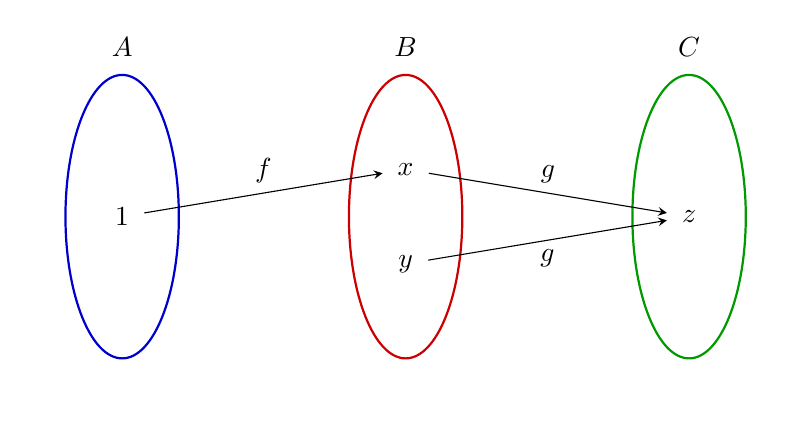
\begin{tikzpicture}[scale=1.2]
    % Background fill for safety
    \fill[white] (-1,-2) rectangle (7,2);
    
    % Sets
    \draw[thick, blue!80!black] (0,0) ellipse (0.6 and 1.5);
    \draw[thick, red!80!black] (3,0) ellipse (0.6 and 1.5);
    \draw[thick, green!60!black] (6,0) ellipse (0.6 and 1.5);
    
    % Nodes
    \node at (0, 1.8) {$A$};
    \node at (3, 1.8) {$B$};
    \node at (6, 1.8) {$C$};
    
    \node (a1) at (0,0) {$1$};
    \node (b1) at (3,0.5) {$x$};
    \node (b2) at (3,-0.5) {$y$};
    \node (c1) at (6,0) {$z$};
    
    % Arrows
    \draw[->, >=stealth, shorten >=2pt, shorten <=2pt] (a1) -- (b1) node[midway, above] {$f$};
    \draw[->, >=stealth, shorten >=2pt, shorten <=2pt] (b1) -- (c1) node[midway, above] {$g$};
    \draw[->, >=stealth, shorten >=2pt, shorten <=2pt] (b2) -- (c1) node[midway, below] {$g$};
\end{tikzpicture}
\end{center}
\hfill $\blacksquare$

\vspace{1em}
\textbf{Problem 25:} \textbf{Quant Finance:} Let $(\Omega, \F, \Prob)$ be a probability space. A stock price $S_T: \Omega \to \R$ is a measurable function. A European Put Option payoff is $P(\omega) = \max(K - S_T(\omega), 0)$. Prove that the event ``the option expires in the money'' (i.e., $P(\omega) > 0$) is a measurable set in $\F$.

\textbf{Solution:}
\textit{Proof:} The event is $E = \{\omega \in \Omega : P(\omega) > 0\}$.
Substitute the payoff function: $E = \{\omega \in \Omega : \max(K - S_T(\omega), 0) > 0\}$.
The maximum of $K - S_T(\omega)$ and $0$ is strictly greater than $0$ if and only if $K - S_T(\omega) > 0$.
This is equivalent to $S_T(\omega) < K$.
Thus, $E = \{\omega \in \Omega : S_T(\omega) \in (-\infty, K)\}$.
By definition of the preimage, $E = S_T^{-1}((-\infty, K))$.
Since $S_T$ is a measurable function (a random variable), the preimage of any Borel set in $\R$ must belong to the $\sigma$-algebra $\F$. The open interval $(-\infty, K)$ is a Borel set. Therefore, $S_T^{-1}((-\infty, K)) \in \F$. \hfill $\blacksquare$

\vspace{1em}
\textbf{Problem 26:} \textbf{Quant Finance:} Let $V_0 = e^{-rT} \E^\Q[\max(S_T - K, 0)]$. Suppose $S_T(\omega) = K$ for all $\omega \in \Omega$. Rigorously evaluate $V_0$ and interpret the preimage $S_T^{-1}(\{K\})$.

\textbf{Solution:}
If $S_T(\omega) = K$ for all $\omega \in \Omega$, then the payoff function is $C(\omega) = \max(K - K, 0) = 0$ for all $\omega$.
The expected value of a constant $0$ random variable under any probability measure $\Q$ is $0$.
Thus, $V_0 = e^{-rT} \cdot 0 = 0$.
The preimage $S_T^{-1}(\{K\}) = \{\omega \in \Omega : S_T(\omega) = K\}$. Since $S_T(\omega) = K$ for all $\omega$, this preimage is the entire sample space $\Omega$. In probability terms, the event that the stock price equals the strike price is a certain event, $\Q(\Omega) = 1$. \hfill $\blacksquare$

\vspace{1em}
\textbf{Problem 27:} \textbf{Machine Learning:} Let a neural network be modeled as $f_\theta: \R^n \to \R^m$. The loss function is $L(\theta) = \|f_\theta(x) - y\|^2$. Prove that if $f_\theta$ is an injective function with respect to $\theta$, then the preimage $L^{-1}(\{0\})$ contains at most one parameter vector $\theta$.

\textbf{Solution:}
\textit{Proof by Contradiction:} Assume $L^{-1}(\{0\})$ contains at least two distinct parameter vectors, $\theta_1$ and $\theta_2$ ($\theta_1 \neq \theta_2$).
By definition of the preimage, $L(\theta_1) = 0$ and $L(\theta_2) = 0$.
This implies $\|f_{\theta_1}(x) - y\|^2 = 0 \implies f_{\theta_1}(x) = y$.
Similarly, $\|f_{\theta_2}(x) - y\|^2 = 0 \implies f_{\theta_2}(x) = y$.
Therefore, $f_{\theta_1}(x) = f_{\theta_2}(x)$.
Since $f_\theta$ is injective with respect to $\theta$, $f_{\theta_1}(x) = f_{\theta_2}(x)$ implies $\theta_1 = \theta_2$.
This contradicts our assumption that $\theta_1 \neq \theta_2$. Thus, the preimage contains at most one element. \hfill $\blacksquare$

\vspace{1em}
\textbf{Problem 28:} \textbf{Machine Learning:} Let $\sigma(x) = \frac{1}{1 + e^{-x}}$ be the sigmoid activation function. Prove that $\sigma: \R \to (0, 1)$ is a bijection, and find its inverse function.

\textbf{Solution:}
\textit{Injectivity:} Assume $\sigma(x_1) = \sigma(x_2)$.
\[ \frac{1}{1 + e^{-x_1}} = \frac{1}{1 + e^{-x_2}} \implies 1 + e^{-x_1} = 1 + e^{-x_2} \implies e^{-x_1} = e^{-x_2} \]
Taking the natural logarithm of both sides yields $-x_1 = -x_2 \implies x_1 = x_2$. Thus, $\sigma$ is injective.
\textit{Surjectivity \& Inverse:} Let $y \in (0, 1)$. Set $y = \frac{1}{1 + e^{-x}}$ and solve for $x$:
\[ 1 + e^{-x} = \frac{1}{y} \implies e^{-x} = \frac{1}{y} - 1 = \frac{1 - y}{y} \]
Since $y \in (0, 1)$, $1 - y > 0$ and $y > 0$, so $\frac{1 - y}{y} > 0$. We can take the natural logarithm:
\[ -x = \ln\left(\frac{1 - y}{y}\right) \implies x = -\ln\left(\frac{1 - y}{y}\right) = \ln\left(\frac{y}{1 - y}\right) \]
Since $x \in \R$ exists for every $y \in (0, 1)$, $\sigma$ is surjective. The inverse function is $\sigma^{-1}(y) = \ln\left(\frac{y}{1 - y}\right)$, known as the logit function. \hfill $\blacksquare$

\vspace{1em}
\textbf{Problem 29:} \textbf{Find the Flaw:} \textit{Claim:} The function $f: \R \to \R$ defined by $f(x) = x^2$ is injective. \textit{Proof:} Let $x, y \in \R$ and assume $x = y$. Squaring both sides gives $x^2 = y^2$, which means $f(x) = f(y)$. Therefore, $f$ is injective. Identify the logical flaw.

\textbf{Solution:}
\textit{The Flaw:} The proof verifies that the relation is a \textit{function} (well-defined), not that it is injective. The definition of injectivity requires assuming $f(x) = f(y)$ and proving $x = y$. The proof assumes $x = y$ and proves $f(x) = f(y)$, which is the converse statement. A correct counterexample to injectivity is $f(2) = 4$ and $f(-2) = 4$, but $2 \neq -2$. \hfill $\blacksquare$

\vspace{1em}
\textbf{Problem 30:} \textbf{Find the Flaw:} \textit{Claim:} For any function $f: A \to B$ and subsets $X, Y \subseteq A$, $f(X \setminus Y) \subseteq f(X) \setminus f(Y)$. \textit{Proof:} Let $b \in f(X \setminus Y)$. Then there exists $a \in X \setminus Y$ such that $f(a) = b$. Since $a \in X$, $f(a) \in f(X)$. Since $a \notin Y$, $f(a) \notin f(Y)$. Thus $b \in f(X) \setminus f(Y)$. Identify the logical flaw.

\textbf{Solution:}
\textit{The Flaw:} The statement ``Since $a \notin Y$, $f(a) \notin f(Y)$'' is logically invalid unless $f$ is injective. It is entirely possible that $a \notin Y$, but there exists some other element $y \in Y$ such that $f(a) = f(y)$. In that case, $f(a)$ \textit{would} be in $f(Y)$. For example, let $f(x) = x^2$, $X = \{2\}$, $Y = \{-2\}$. $X \setminus Y = \{2\}$. $f(X \setminus Y) = \{4\}$. But $f(X) = \{4\}$ and $f(Y) = \{4\}$, so $f(X) \setminus f(Y) = \emptyset$. Clearly $\{4\} \not\subseteq \emptyset$. \hfill $\blacksquare$

\newpage

\section{Concept Checklist \& Question Mapping (Repeated)}

\renewcommand{\arraystretch}{1.5}
\begin{tabularx}{\textwidth}{>{\raggedright\arraybackslash}p{1.5cm} >{\raggedright\arraybackslash}X >{\raggedright\arraybackslash}p{3.5cm}}
\toprule
\textbf{ID} & \textbf{Concept / Logical Structure} & \textbf{Associated Problems} \\
\midrule
C1 & Relation vs. Function (Existence \& Uniqueness) & 1, 2, 3, 4 \\
C2 & Domain and Range Computations (Algebraic Inversion) & 5, 6, 7, 8 \\
C3 & Image and Preimage Properties (Set-Theoretic Proofs) & 9, 10, 11, 12 \\
C4 & Cardinality of Function Spaces ($|B^A|$) & 13, 14, 15 \\
C5 & Higher-Order Functions and Functionals ($C^{B^A}$) & 16, 17, 18 \\
C6 & Injectivity, Surjectivity, and Bijectivity & 19, 20, 21 \\
C7 & Composition of Functions & 22, 23, 24 \\
C8 & Abstract Real-World Modeling (Quant Finance \& ML) & 25, 26, 27, 28 \\
C9 & Flaw Identification / Diagnostic Logic & 29, 30 \\
\bottomrule
\end{tabularx}

\end{document}